\documentclass[10pt, landscape]{article}
\usepackage[scaled=0.92]{helvet}
\usepackage{calc}
\usepackage{multicol}
\usepackage{ifthen}
\usepackage[a4paper,margin=3mm,landscape]{geometry}
\usepackage{amsmath,amsthm,amsfonts,amssymb}
\usepackage{color,graphicx,overpic}
\usepackage{hyperref}
\usepackage{newtxtext} 
\usepackage{enumitem}
\usepackage{amssymb}
\usepackage[table]{xcolor}
\usepackage{vwcol}
\usepackage{tikz}
\usepackage{wrapfig}
\usepackage{makecell}
\setlist{nosep}
\graphicspath{ {./images/} }

\pdfinfo{
  /Title (MA1521-cheatsheet.pdf)
  /Creator (Jovyn)
  /Producer (pdfTeX 1.40.0)
  /Author (Jovyn)
  /Subject (MA1521)
  /Keywords (ma1521, cheatsheet, tex)}

% Turn off header and footer
\pagestyle{empty}

% for tight centres (less spacing)
\newenvironment{tightcenter}{%
  \setlength\topsep{0pt}
  \setlength\parskip{0pt}
  \begin{center}
}{%
  \end{center}
}

% redefine section commands to use less space
\makeatletter
\renewcommand{\section}{\@startsection{section}{1}{0mm}%
                                {-1ex plus -.5ex minus -.2ex}%
                                {0.5ex plus .2ex}%x
                                {\normalfont\large\bfseries}}
\renewcommand{\subsection}{\@startsection{subsection}{2}{0mm}%
                                {-1explus -.5ex minus -.2ex}%
                                {0.5ex plus .2ex}%
                                {\normalfont\normalsize\bfseries}}
\renewcommand{\subsubsection}{\@startsection{subsubsection}{3}{0mm}%
                                {-1ex plus -.5ex minus -.2ex}%
                                {1ex plus .2ex}%
                                {\normalfont\small\bfseries}}%
\renewcommand{\familydefault}{\sfdefault}
\renewcommand\rmdefault{\sfdefault}
% makes nested numbering (e.g. 1.1.1, 1.1.2, etc)
\renewcommand{\labelenumii}{\theenumii}
\renewcommand{\theenumii}{\theenumi.\arabic{enumii}.}
\renewcommand\labelitemii{•}
%  for logical not operator
\renewcommand{\lnot}{\mathord{\sim}}
\renewcommand{\bf}[1]{\textbf{#1}}
\newcommand{\abs}[1]{\vert #1 \vert}
\newcommand{\Mod}[1]{\ \mathrm{mod}\ #1}
\newcommand{\vv}[1]{\boldsymbol{#1}}
\newcommand{\VV}[1]{\overrightarrow{#1}}
\newcommand{\cvv}[1]{\left(\begin{smallmatrix}#1\end{smallmatrix}\right)}

\makeatother
\definecolor{myblue}{cmyk}{1,.72,0,.38}
% Define BibTeX command
\everymath\expandafter{\the\everymath \color{myblue}}
\def\BibTeX{{\rm B\kern-.05em{\sc i\kern-.025em b}\kern-.08em
    T\kern-.1667em\lower.7ex\hbox{E}\kern-.125emX}}
\let\iff\leftrightarrow
\let\Iff\Leftrightarrow
\let\then\rightarrow
\let\Then\Rightarrow

% Don't print section numbers
\setcounter{secnumdepth}{0}

\setlength{\parindent}{0pt}
\setlength{\parskip}{0pt plus 0.5ex}
%% this changes all items (enumerate and itemize)
\setlength{\leftmargini}{0.5cm}
\setlength{\leftmarginii}{0.5cm}
\setlist[itemize,1]{leftmargin=2mm,labelindent=1mm,labelsep=1mm}
\setlist[itemize,2]{leftmargin=4mm,labelindent=1mm,labelsep=1mm}

%My Environments
\newtheorem{example}[section]{Example}
% -----------------------------------------------------------------------

\begin{document}
\raggedright
\footnotesize
\begin{multicols*}{4}


% multicol parameters
% These lengths are set only within the two main columns
\setlength{\columnseprule}{0.25pt}
\setlength{\premulticols}{1pt}
\setlength{\postmulticols}{1pt}
\setlength{\multicolsep}{1pt}
\setlength{\columnsep}{2pt}

\begin{center}
    \fbox{%
        \parbox{0.8\linewidth}{\centering \textcolor{black}{
            {\Large\textbf{MA1521}}
            \\ \normalsize{AY20/21 Sem 1}}
            \\ {\footnotesize by jovyntls}
        }%
    }
\end{center}

\section{01. FUNCTIONS \& LIMITS}
\subsection{Rules of Limits}
\begin{enumerate}
    \item $\lim\limits_{x\to{a}}(f\pm g)(x) = L \pm L'$
    \item $\lim\limits_{x\to{a}}(fg)(x) = LL'$
    \item $\lim\limits_{x\to{a}}\frac{f}{g}(x) = \frac{L}{L'}$, provided $L'\neq 0$
    \item $\lim\limits_{x\to{a}}kf(x) = kL${ for any real number }$k.$
\end{enumerate}

% \subsection{Estimation}
% first order estimate: 
% $y' \approx y + \Delta x \times \frac{dy}{dx} \Bigr|_{x=2}$

% second order estimate: 
% $y' \approx \text{1st estimate } + (\frac{(\triangle x)^2}{2}\times\frac{d^2y}{dx^2}\Bigr|_{x=2})$

% \subsection{Stats}
% pop. variance:
% $\sigma ^2=\frac{\sum x^2-\frac{(\sum x)^2}{n}}{n}$

% pop. covariance: 
% $\text{cov}(x, y) =\frac{\sum xy^2 - \frac{\sum x \sum y}{n}}{n}$

% pop. correlation: 
% $\frac{\text{cov}(x, y)}{\sigma_x \times \sigma_y}$


\section{02. DIFFERENTIATION}
extreme values:
\begin{itemize}
    \item $f'(x)=0$
    \item $f'(x)$ does not exist
    \item end points of the domain of $f$
\end{itemize}
parametric differentiaton: $\frac{d^2y}{dx^2} = \frac{d}{dx}(\frac{dy}{dx}) = \frac{\frac{d}{dt}(\frac{dy}{dx})}{\frac{dx}{dt}}$

\subsection{Differentiation Techniques}
\begin{center}
    \begin{tabular}{|>{\color{black}}c | >{\color{black}}c|}
        \hline
        $f(x)$ & $f'(x)$
        \\ \hline
        \rule{0pt}{2.3ex}  % top spacing
            $\tan x$ & $\sec ^2 x$ \\
            $\csc x$ & $-\csc x \cot x$ \\
            $\sec x$ & $\sec x \tan x$ \\
            $\cot x$ & $- \csc ^2 x$
        \\ \hline
        \rule{0pt}{2.3ex}  % top spacing
            $a^{f(x)}$ & $\ln a \cdot f'(x)a^{f(x)}$ \\
            $\log_af(x)$ & $\log_a e \cdot \frac{f'(x)}{f(x)}$
        \\[1ex] \hline
        \rule{0pt}{3ex}  % top spacing
            $\sin^{-1} f(x)$ & $\frac{f'(x)}{\sqrt{1-[f(x)]^2}}, \ \ _{\vert f(x) \vert < 1}$ \\[1.5ex]
            $\cos^{-1} f(x)$ & $-\frac{f'(x)}{\sqrt{1-[f(x)]^2}}, \ \ _{\vert f(x) \vert < 1}$ \\[1.5ex]
            $\tan^{-1} f(x)$ & $\frac{f'(x)}{1 + [f(x)]^2}$ \\[1.5ex]
            $\cot^{-1} f(x)$ & $-\frac{f'(x)}{1 + [f(x)]^2}$ \\[1.5ex]
            $\sec^{-1} f(x)$ & $\frac{f'(x)}{\vert f(x) \vert \sqrt{[f(x)]^2-1}}$ \\[1.5ex]
            $\csc^{-1} f(x)$ & $-\frac{f'(x)}{\vert f(x) \vert \sqrt{[f(x)]^2-1}}$ \\[2ex]
        \hline
    \end{tabular}
\end{center}

\subsection{L'Hopital's Rule}
\begin{center}
    $\lim\limits_{x\to x_0}\frac{f(x)}{g(x)}=\lim\limits_{x\to x_0}\frac{f'(x)}{g'(x)}$
\end{center}
\begin{itemize}
    \item for indeterminate forms ($\frac{0}{0}$ or $\frac{\infty}{\infty}$), cannot directly substitute $x=a$. \\*
    \item for other forms: convert to ($\frac{0}{0}$ or $\frac{\infty}{\infty}$) then apply L'Hopital's rule \\*
    \item for exponents: use $\ln$, then sub into $e^{f(x)}$
\end{itemize}


\section{03. INTEGRATION}
\subsection{Integration Techniques}
\begin{center}
    \def\arraystretch{1.2}
    \begin{tabular}{|>{\color{black}}c | >{\color{black}}c|}
        \hline
        $f(x)$ & $\int f(x)$
        \\ \hline
            $\tan x$ & $\ln (\sec x),$ \tiny{${\vert x \vert < \frac{\pi}{2}}$} \\
            $\cot x$ & $\ln (\sin x),$ \tiny{$0 < x < \pi $} \\
            $\csc x$ & $-\ln (\csc x + \cot x),$ \tiny{$0 < x < \pi $} \\
            $\sec x$ & $\ln (\sec x + \tan x),$ \tiny{$\vert x \vert < \frac{\pi}{2} $}
        \\[0.5ex] \hline
        \rule{0pt}{2.3ex}  % top spacing
            $\frac{1}{x^2 + a^2}$ & $\frac{1}{a} \tan^{-1}(\frac{x}{a})$ \\
            $\frac{1}{\sqrt{a^2 - x^2}}$ & $\sin^{-1}(\frac{x}{a})$, \tiny{$\vert x \vert < a$} \\
            $\frac{1}{x^2 - a^2}$ & $\frac{1}{2a} \ln(\frac{x - a}{x + a})$, \tiny{$x > a$} \\[1ex]
            $\frac{1}{a^2 - x^2}$ & $\frac{1}{2a} \ln(\frac{x + a}{x - a})$, \tiny{$x < a$} 
        \\[0.5ex] \hline 
        \rule{0pt}{2.6ex}  % top spacing
            $a^{x}$ & $\frac{a^x}{\ln a}$ \\[0.5ex]
        \hline
    \end{tabular}
\end{center}

\begin{center}
    $\frac{d}{dx}\int^x_af(t)dt = f(x)$
\end{center}
\begin{itemize}
    \item \textbf{indefinite integral} — the integral of the function without any limits
    \item \textbf{antiderivative} — any function whose derivative will be the same as the original function
\end{itemize}
substitution: $\int^b_af\big (g(x)\big )g'(x)dx = \int^{g(b)}_{g(a)}f(u)du$ \\*
by parts: $\int uv'\ dx = uv - \int u'v\ dx$ \\*
\subsection{Volume of Revolution}
about x-axis:
\begin{itemize}
    \item (with hollow area) $V = \pi\int^b_a [f(x)]^2 - [g(x)]^2dx$
    \item (about line $y=k$) $V = \pi\int^b_a [f(x) - k]^2dx$
\end{itemize}

\section{04. SERIES}
\subsection{Geometric Series}
\begin{center}
    \begin{multicols}{2}
        sum (\textbf{divergent}) 
        \\* $\frac{a(1-r^n)}{1-r}$
        
        sum (\textbf{convergent}) 
        \\* $\frac{a}{1-r}$
    \end{multicols}
\end{center}

\subsection{Power Series}
\begin{center}
    power series about $x = 0$
    $\sum\limits^\infty_{n=0}c_nx^n = c_0 + c_1x + c_2x^2 + \dots$

    power series about $x = a$ ($a$ is the centre of the power series)
    $\sum\limits^\infty_{n=0}c_nx^n = c_0 + c_1(x-a) + c_2(x-a)^2 + \dots$
\end{center}

\subsection{Taylor series}
\begin{center}
    $\sum\limits^\infty_{k = 0} \frac{f^k(a)}{k!}(x-a)^k$

    MacLaurin series:
    \\* $f(x) = \sum\limits^\infty_{n=0}\frac{f^n(0)}{n!}x^n$

    Taylor polynomial of $f$ at $a$:
    \\* $P_n(x) = \sum\limits^n_{k = 0} \frac{f^k(a)}{k!} (x-a)^k$
\end{center}

\subsubsection{Radius of Convergence}
power series converges where $\lim\limits_{n \to \infty} \abs{\frac{u_{n+1}}{u_n}} < 1$
\begin{center}
    \begin{tabular}{| p{0.25\linewidth} | p{0.15\linewidth} | p{0.35\linewidth} |} 
        \hline
        converge at
        & $R$
        & $\lim\limits_{n \to \infty} \abs{\frac{u_{n+1}}{u_n}}$ \\
        \hline
        $x = a$ & $0$ & $\infty$
        \\ \hline 
        $(x - h, x + h)$ & $h, \frac{1}{N}$ & $N \cdot \abs{x - a}$
        \\ \hline 
        all $x$ & $\infty$ & $0$
        \\ \hline 
    \end{tabular} 
\end{center}

\subsection{MacLaurin Series}
For $-\infty < x < \infty$
\\ \;  % spacing
\setlength\tabcolsep{1.5pt} % default value: 6pt
\begin{tabular}{rl}
           $\sin x$ & $= \sum\limits^\infty_{n = 0} \frac{(-1)^nx^{2n + 1}}{(2n+1)!} $
        \\ $\cos x$ & $= \sum\limits^\infty_{n = 0} \frac{(-1)^nx^{2n}}{(2n)!}$
        \\ $e^x$ & $= \sum\limits^\infty_{n = 0} \frac{x^n}{n!}$
\end{tabular}

For $-1 < x < 1$
\\ \;  % spacing
\setlength\tabcolsep{1.5pt} % default value: 6pt
\begin{tabular}{rl}
           $\frac{1}{1 - x}$ & $= \sum\limits^\infty_{n = 0} x^n $
        \\ $\frac{1}{1 + x}$ & $= \sum\limits^\infty_{n = 0} (-1)^nx^n $
        \\ $\frac{1}{1 + x^2}$ & $= \sum\limits^\infty_{n = 0} (-1)^nx^{2n} $
        \\ $\ln(1 + x)$ & $= \sum\limits^\infty_{n = 1} \frac{(-1)^{n - 1}x^n}{n} $
        \\ $\tan^{-1}x$ & $= \sum\limits^\infty_{n = 0} \frac{(-1)^n}{2n + 1} x^{2n+1}$
        \\ $\frac{1}{(1+x)^2}$ & $= \sum\limits^\infty_{n = 1} (-1)^{n-1}nx^{n-1}$
        \\ $\frac{1}{(1-x)^2}$ & $= \sum\limits^\infty_{n = 1} nx^{n-1}$
        \\ $\frac{1}{(1-x)^3}$ & $= \frac{1}{2} \sum\limits^\infty_{n = 2} n(n - 1)x^{n-2}$
        \\ $(1 + x)^k$ & $= \sum\limits^\infty_{n = 0} \binom{k}{n}x^n$
        \\   & $= 1 + kx + \frac{k(k-1)}{2!}x^2 + \dots$
\end{tabular}

\subsubsection{Differentiation/Integration}
\begin{center}
    For $f(x) = \sum\limits^\infty_{n = 0}c_n(x - a)^n$\  and \ $a-h<x<a+h$,
    \textbf{differentiation} of power series:
    \\* $f'(x) = \sum\limits^\infty_{n = 0}nc_n(x-a)^{n-1}$
    
    \textbf{integration} of power series:
    \\* $\int f(x) dx = \sum\limits^\infty_0c_n \frac{(x - 1)^{n + 1}}{n + 1} + c$
    \\* if $R=\infty$, $f(x)$ can be integrated to $\int^1_0 f(x) dx$
\end{center}

\section{05. VECTORS}
unit vector, $\hat{\vv{p}} = \frac{\vv{p}}{\abs{\vv{p}}}$
\begin{center}
    \begin{multicols}{2}
        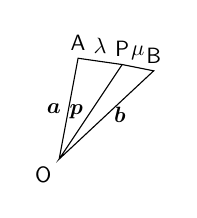
\begin{tikzpicture}[scale=0.8, every node/.style={transform shape}]
            \coordinate[label=below left:O] (O) at (0,0);
            \coordinate[label=A] (A) at (0.3,1.6);
            \coordinate[label=B] (B) at (1.5, 1.4);
            \coordinate[label=P] (P) at (1, 1.5);
            \draw (O) 
            -- node[left] {$\vv{a}$} (A) 
            -- node[above] {$\lambda$} (P)
            -- node[above] {$\mu$} (B) 
            -- node[right] {$\vv{b}$} (O) 
            -- node[left] {$\vv{p}$} (P);
        \end{tikzpicture}
        \\ \textbf{ratio theorem}
        \\* $\vv{p} = \frac{\mu\vv{a} + \lambda\vv{b}}{\lambda + \mu}$
        \newline
        \\ \textbf{midpoint theorem}
        \\* $\vv{p} = \frac{\vv{a} + \vv{b}}{2}$
    \end{multicols}
\end{center}

\subsection{Dot product}
\begin{center}
    $\vv{a} \cdot \vv{b} = \abs{\vv{a}} \abs{\vv{b}} \cos \theta$
    \\* $\cvv{a_1 \\ a_2 \\ a_3} \cdot \cvv{b_1 \\ b_2 \\ b_3} = a_1b_1 + a_2b_2 + a_3b_3$
    \newline
    \begin{multicols}{2}
        $\vv{a} \perp \vv{b} \Then \vv{a} \cdot \vv{b} = 0$
        \\ $\vv{a} \parallel \vv{b} \Then \vv{a} \cdot \vv{b} = \abs{\vv{a}} \abs{\vv{b}}$
        \\ $\vv{a} \cdot \vv{b} > 0$ : $\vv{a}$ is acute
        \\ $\vv{a} \cdot \vv{b} < 0$ : $\vv{a}$ is obtuse
    \end{multicols}
\end{center}

\subsection{Cross product}
\begin{center}
    $\vv{a} \times \vv{b} = \abs{\vv{a}} \abs{\vv{b}} \sin \theta \hat{\vv{n}}$
    \\* $\cvv{a_1 \\ a_2 \\ a_3} \cdot \cvv{b_1 \\ b_2 \\ b_3} 
        = \cvv{a_2b_3 - 1_3b_2 \\ -(a_1b_3 - a_3b_1) \\ a_1b_2 - a_2b_1}$
    \newline
    \begin{multicols}{2}
        $\vv{a} \perp \vv{b} \Then \vv{a} \times \vv{b} = \abs{\vv{a}} \abs{\vv{b}}$
        $\vv{a} \parallel \vv{b} \Then \vv{a} \times \vv{b} = 0$
        $\vv{a} \times \vv{b} = -(\vv{b} \times \vv{a})$
        $\lambda\vv{a} \times \mu\vv{b} = \lambda\mu(\vv{a} \times \vv{b})$
    \end{multicols}
\end{center}

\subsection{Projection}
\begin{multicols}{2}
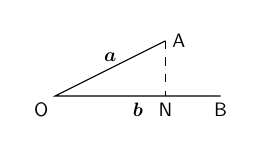
\begin{tikzpicture}[scale=0.7, every node/.style={transform shape}]
    \coordinate[label=below left:O] (O) at (0,0);
    \coordinate[label=right:A] (A) at (2, 1);
    \coordinate[label=below:B] (B) at (3, 0);
    \coordinate[label=below:N] (N) at (2, 0);
    \draw (A) 
        -- node[above] {$\vv{a}$} (O)
        -- node[below] {$\vv{b}$} (B); 
    \draw[shorten >=0pt, dashed] (A) -- (N);
\end{tikzpicture}
$\triangle ANO = \frac{1}{2} \abs{\VV{OA} \times \VV{ON}}$
\begin{center}
    $\abs{\VV{ON}} = \abs{\vv{a} \cdot \hat{\vv{b}}} = \frac{\abs{\vv{a} \cdot \vv{b}}}{\abs{\vv{b}}}$
    \\* $\VV{ON} = (\vv{a} \cdot \hat{\vv{b}})\hat{\vv{b}} = \frac{\abs{\vv{a} \cdot \vv{b}}}{\abs{\vv{b}}^2}\vv{b}$
\end{center}
\end{multicols}

\subsection{Planes}
\subsubsection{Equation of a Plane}
$\vv{n}$ is a perpendicular to the plane; $A$ is a point on the plane.
\begin{itemize}
    \item parametric: $\vv{r} = \vv{a} + \lambda\vv{b} + \mu\vv{c}$
    \item scalar product: $\vv{r} \cdot \vv{n} = \vv{a} \cdot \vv{n}$
    \item standard form: $\vv{r} \cdot \hat{\vv{n}} = d$ 
    \item cartesian: $\vv{a}x + \vv{b}y + \vv{c}z = p$
\end{itemize}
Length of projection of $\vv{a}$ on $\vv{n} = \abs{\vv{a} \cdot \hat{\vv{n}}} = \perp$ from $O$ to $\pi$

\subsubsection{Distance from a point to a plane}
\begin{center}
    Shortest distance from a point $S(x_0, y_0, z_0)$ to a plane $\Pi: ax + by + c = d$ is given by:
    \\* $\frac{\abs{ax_0 + by_0 + cz_0 - d}}{\sqrt{a^2 + b^2 + c^2}}$
\end{center}

\section{06. PARTIAL DIFFERENTIATION}
\subsection{Partial Derivatives}
For $f(x, y)$,
\begin{center}
    first-order partial derivatives:
    \begin{multicols}{2}
            $f_x = \frac{d}{dx}f(x, y)$
            \\ $f_y = \frac{d}{dy}f(x, y)$
    \end{multicols}

    second-order partial derivatives:
    \begin{multicols}{2}
            $f_{xx} = (f_x)_x = \frac{d}{dx}f_x$
            \\ $f_{yy} = (f_y)_y = \frac{d}{dy}f_y$
            \\ $f_{xy} = (f_x)_y = \frac{d}{dy}f_x$
            \\ $f_{yx} = (f_y)_x = \frac{d}{dx}f_y$
    \end{multicols}
\end{center}

\subsection{Chain Rule}
\begin{center}
    For $z(t) = f(x(t), y(t))$,
    \\* $\frac{dz}{dt} = \frac{\partial z}{\partial x} \frac{dx}{dt} + \frac{\partial z}{\partial y} \frac{dy}{dt}$

    For $z(s, t) = f\big(x(s, t), y(s, t)\big)$,
    \\ $\frac{\partial z}{\partial t} = \frac{\partial z}{\partial x} \frac{\partial x}{\partial t} + \frac{\partial z}{\partial y} \frac{\partial y}{\partial t}$
    \\ $\frac{\partial z}{\partial s} = \frac{\partial z}{\partial x} \frac{\partial x}{\partial s} + \frac{\partial z}{\partial y} \frac{\partial y}{\partial s}$
\end{center}

\subsection{Directional Derivatives}
\begin{center}
    The directional derivative of $f$ at $(a, b)$ in the direction of unit vector $\hat{\vv{u}} = u_1\vv{i} + u_2\vv{j}$ is 
    $D_uf(a, b) = f_x(a, b) \cdot u_1 + f_y(a, b) \cdot u_2$
\end{center}

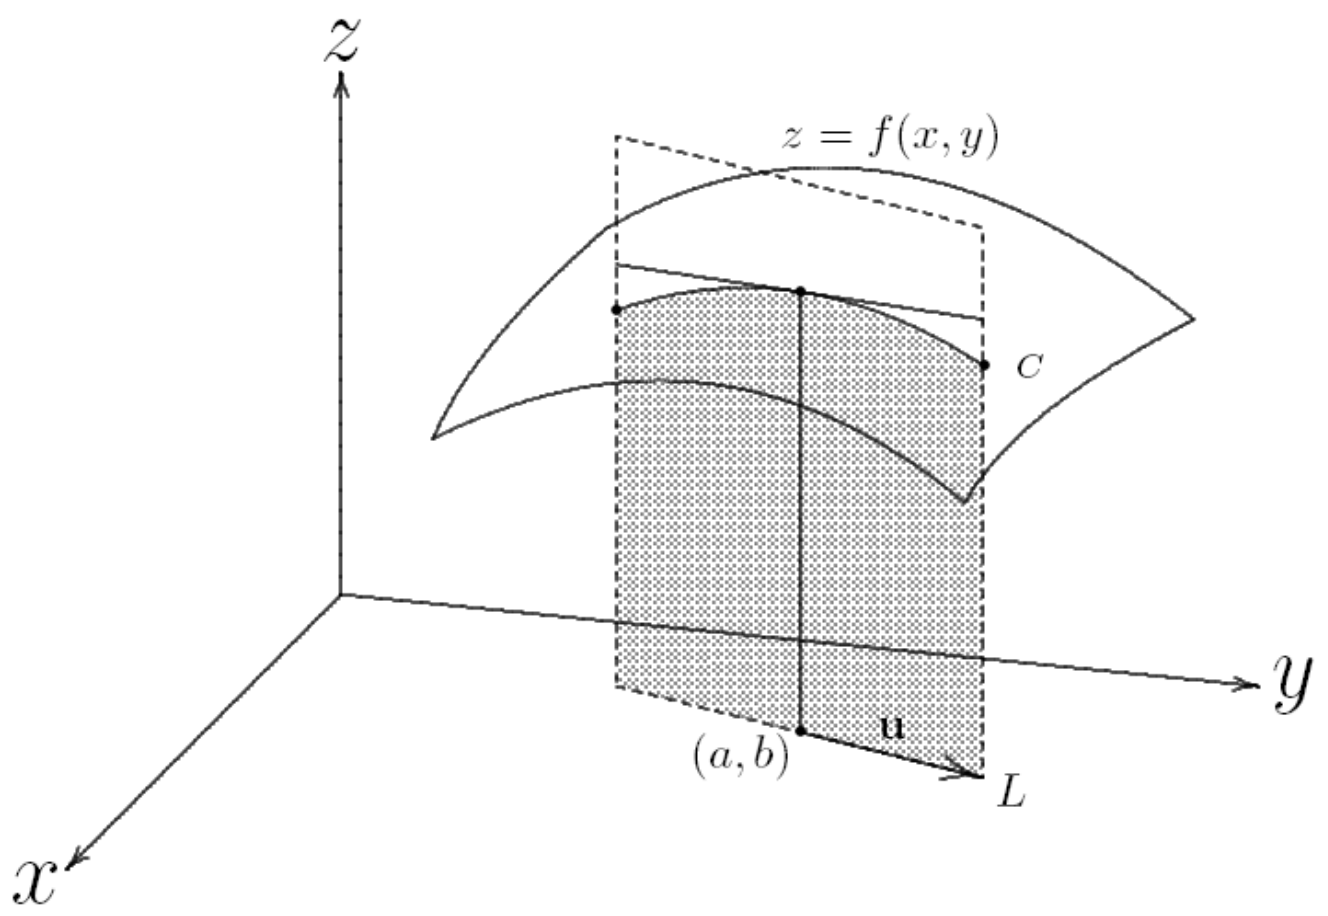
\includegraphics[width=0.8\linewidth]{MA1521-ch6-fig1}

\begin{itemize}
    \item \textbf{geometric meaning}: $D_uf(a, b)$ is the gradient of the tangent at $(a, b)$ to curve $C$ on a surface $z= f(x, y)$
    \begin{itemize}
        \item rate of change of $f(x, y)$ at $(a, b)$ in the direction of $\vv{u}$
    \end{itemize}
\end{itemize}

% \begin{center}
%     $x = a + u_1t, y = b + u_2t, z=0$
%     \\* $D_if(a, b) = f_x(a, b)$
%     \\* $D_jf(a, b) = f_y(a, b)$
% \end{center}

\subsubsection{Gradient Vector}
\begin{center}
    The \textbf{gradient} at $f(x, y)$ is the vector 
    \\* $\nabla f = f_x\vv{i} + f_y\vv{j}$
    \begin{align*}
        D_uf(a, b) &= \nabla f(a, b) \cdot \hat{\vv{u}}
        \\ &= \abs{\nabla f(a, b)} \cos\theta
    \end{align*}
\end{center}
\begin{itemize}
    \item $f$ increases most rapidly in the direction $\nabla f(a, b)$
    \item $f$ decreases most rapidly in the direction $-\nabla f(a, b)$
    \item largest possible value of $D_uf(a, b) = \vert \nabla f(a, b)\vert$
    \begin{itemize}
        \item occurs in the same direction as $f_x(a, b)\vv{i} + f_y(a, b)\vv{j}$
    \end{itemize}
\end{itemize}

\subsubsection{Physical Meaning}
\begin{center}
Suppose a point $p$ moves a small distance $\Delta t$ along a unit vector $\hat{\vv{u}}$ to a new point $\vv{q}$.
\\

\begin{multicols}{2}
    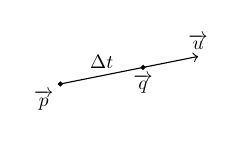
\begin{tikzpicture}[scale=0.7, every node/.style={transform shape}]
        \coordinate[label=below left:$\overrightarrow{p}$] (P) at (0,0);
        \coordinate[label=below:$\overrightarrow{q}$] (Q) at (1.5, 0.3);
        \coordinate[label=$\overrightarrow{u}$] (U) at (2.5, 0.5);
        \filldraw (P) circle (1pt);
        \filldraw (Q) circle (1pt);
        \draw[->] (P) -- node[above] {$\Delta t$} (Q) -- (U);
    \end{tikzpicture}
    \\ increment in $f$, 
    \\* $\Delta f \approx D_uf(\vv{p})(\Delta t)$
\end{multicols}
\end{center}

\subsection{Maximum \& Minimum Values}
$f(x, y)$ has a \textbf{local maximum} at $(a, b)$ if $f(x, y) \leq f(a, b)$ for all points $(x, y)$ near $(a, b)$.
\\ $f(x, y)$ has a \textbf{local minimum} at $(a, b)$ if $f(x, y) \geq f(a, b)$ for all points $(x, y)$ near $(a, b)$.

\subsubsection{Critical Points}
% $f$ has a local maximum/minimum at $(a, b)$ if
\begin{itemize}
    \item $f_x(a, b)$ or $f_y(a, b)$ does not exist; OR
    \item $f_x(a, b) = 0$ and $f_y(a, b) = 0$
    \begin{itemize}
        \item $f_x(0, b) \leq 0$ - maximum point \textit{along the x axis}
        \item $f_y(a, 0) \geq 0$ - minimum point \textit{along the y axis}
    \end{itemize}
\end{itemize}

\subsubsection{Saddle Points}
\begin{itemize}
    \item $f_x(a, b) = 0, f_y(a, b) = 0$
    \item neither a local minimum nor a local maximum
\end{itemize}

\subsubsection{Second Derivative Test}
\begin{center}
    Let $f_x(a, b) = 0$ and $f_y(a, b) = 0$.
    \\* $D = f_{xx}(a, b)f_{yy}(a, b) - f_{xy}(a, b)^2$

    \def\arraystretch{1.2}
    \begin{tabular}{| c | c | c |}
        \hline $D$ & $f_{xx}(a,b)$ & \textbf{local}
        \\\hline + & + & \text{min}
        \\\hline + & - & \text{max}
        \\\hline - & \text{any} & \text{saddle point}
        \\\hline 0 & \text{any} & \text{no conclusion}
        \\\hline
    \end{tabular} 
\end{center}

\section{07. DOUBLE INTEGRALS}
\begin{center}
    Let $\Delta A_i$ be the area of $R_i$ and $(x_i, y_i)$ be a point on $R_i$. 
    \\* Let $f(x, y)$ be a function of two variables. The \textbf{double integral} of $f$ over $R$ is 
    \\* $\displaystyle\iint_R f(x, y) dA = \lim_{n \to \infty} \sum^n_{i=1} f(x_i, y_i) \Delta A_i$
\end{center}

\subsection{Geometric Meaning}
$\iint_R f(x, y) dA$ is the volume under the surface $z = f(x, y)$ and above the $xy$-plane over the region R.
\begin{center}
    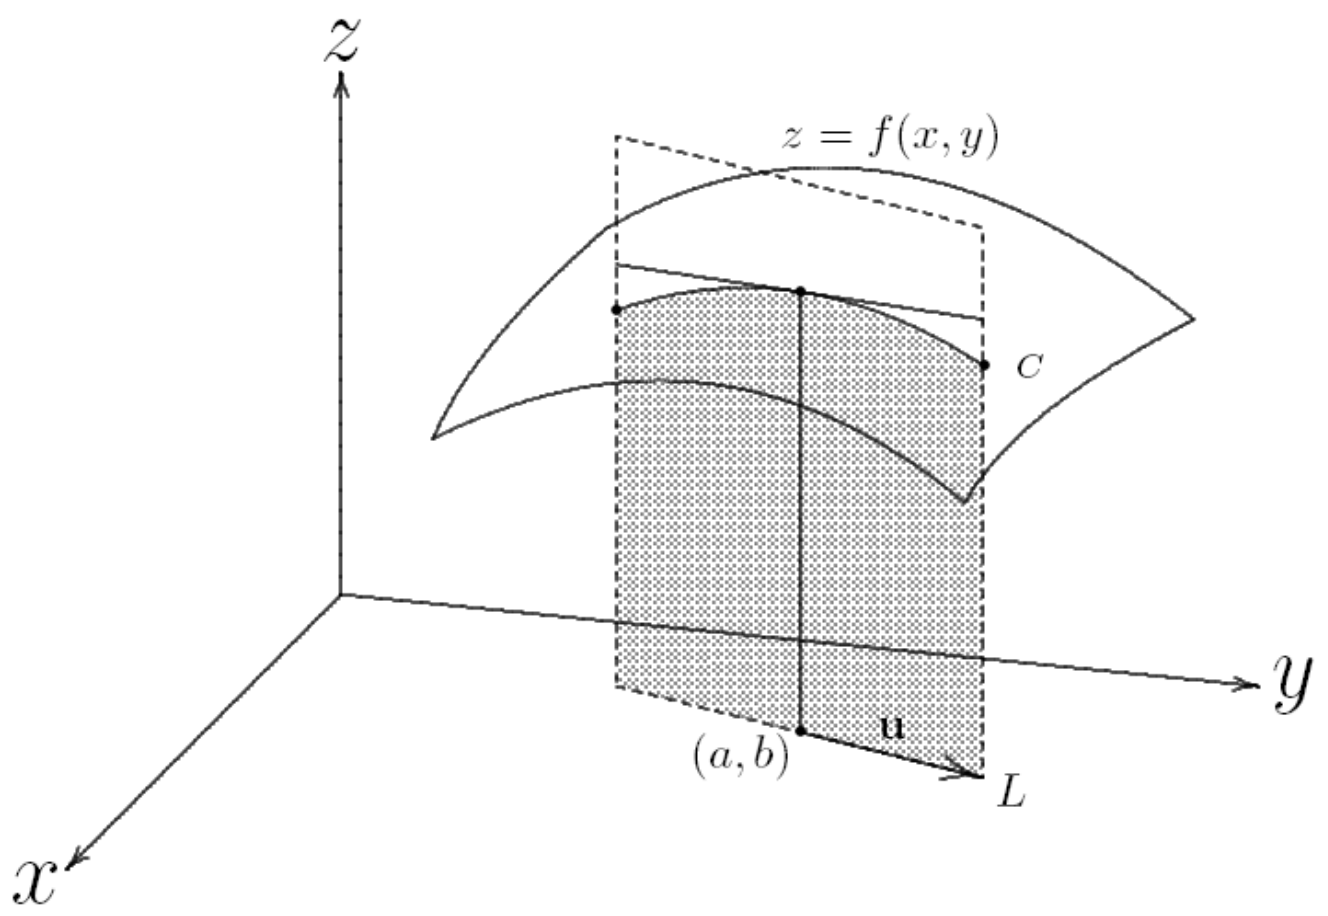
\includegraphics[width=0.7\linewidth]{MA1521-ch7-fig1}
\end{center}

\subsection{Properties of Double Integrals}
\begin{enumerate}
    \item $\iint_R\big(f(x, y) + g(x,y)\big)dA$
        \\ \qquad $ = \iint_Rf(x,y)dA + \iint_Rg(x,y)dA$
    \item $\iint_R cf(x,y)dA = c\iint_R f(x,y)dA$, where $c$ is a constant
    \item If $f(x,y) \geq g(x,y) \text{ for all } (x, y) \in \mathbb{R},$ then 
        \\ \qquad $\iint_R f(x,y)dA \geq \iint_R g(x, y) dA$
    \item If $R$ = $R1 \cup R2$, $R1$ and $R2$ do not overlap, then 
        \\ \centerline{$\iint_R f(x,y) dA = \iint_{R1} f(x,y) dA + \iint_{R2}f(x, y) dA$}
    \item The area of $R$, 
        \\ \qquad $A(R) = \iint_R dA = \iint_R 1 dA$
    \item If $m \leq f(x, y) \leq M$ for all $(x, y) \in R$, then 
        \\ \qquad $mA(R) \leq \iint_R f(x, y)dA \leq MA(R)$
\end{enumerate}

\subsection{Rectangular Regions}
\begin{center}
    For a rectangular region $R$ in the $xy$-plane, $a \leq x \leq b, \quad c \leq y \leq d$
    \begin{align*}
        \iint_R f(x, y) dA &= \int^d_c\left[\int^b_a f(x, y) dx\right]dy
        \\* &= \int^b_a\left[\int^d_c f(x, y) dy\right]dx
    \end{align*}

    If $f(x, y) = g(x) h(y)$, then 
    \\* $\displaystyle \iint_R g(x)h(y)dA = \left(\int^b_a g(x)dx\right) \left(\int^d_c h(y)dy\right)$
\end{center}

\subsection{General Regions}
\subsubsection{Type A}
\begin{center}    
    \begin{multicols}{2}
        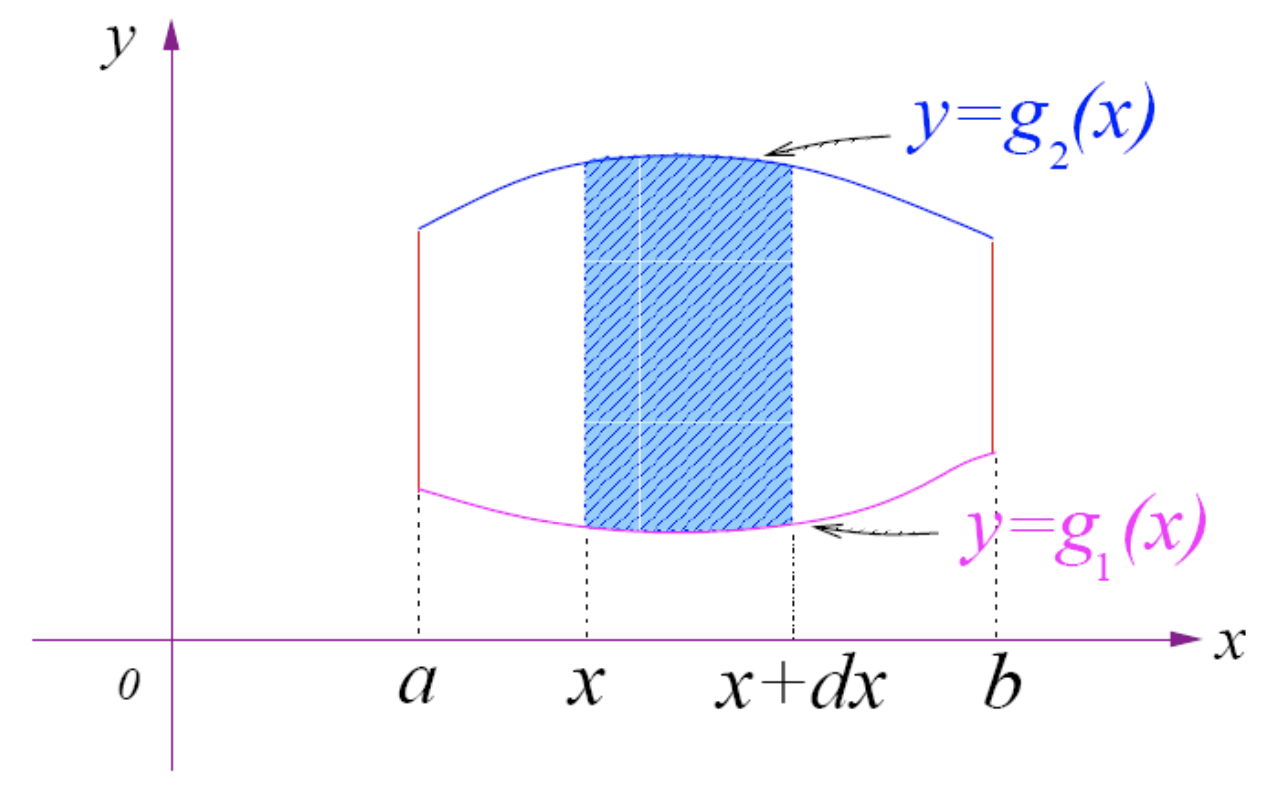
\includegraphics[width=0.9\linewidth]{ma1521-ch7-typeA}
        \\ lower/upper bounds:
        \\* $g_1(x) \leq y \leq g_2(x)$
        \\ \ 
        \\ left/right bounds:
        \\* $a \leq x \leq b$
    \end{multicols}
    
    The region $R$ is given by
    % \\* $R : g_1(x) \leq y \leq g_2(x), \ a \leq x \leq b$
    \\* $\displaystyle\iint_R f(x,y) dA = \int^b_a\Big [ \int^{g_2(x)}_{g_1(x)}f(x,y)dy \Big ]dx$
\end{center}

\subsubsection{Type B}
\begin{center}    
    \begin{multicols}{2}
        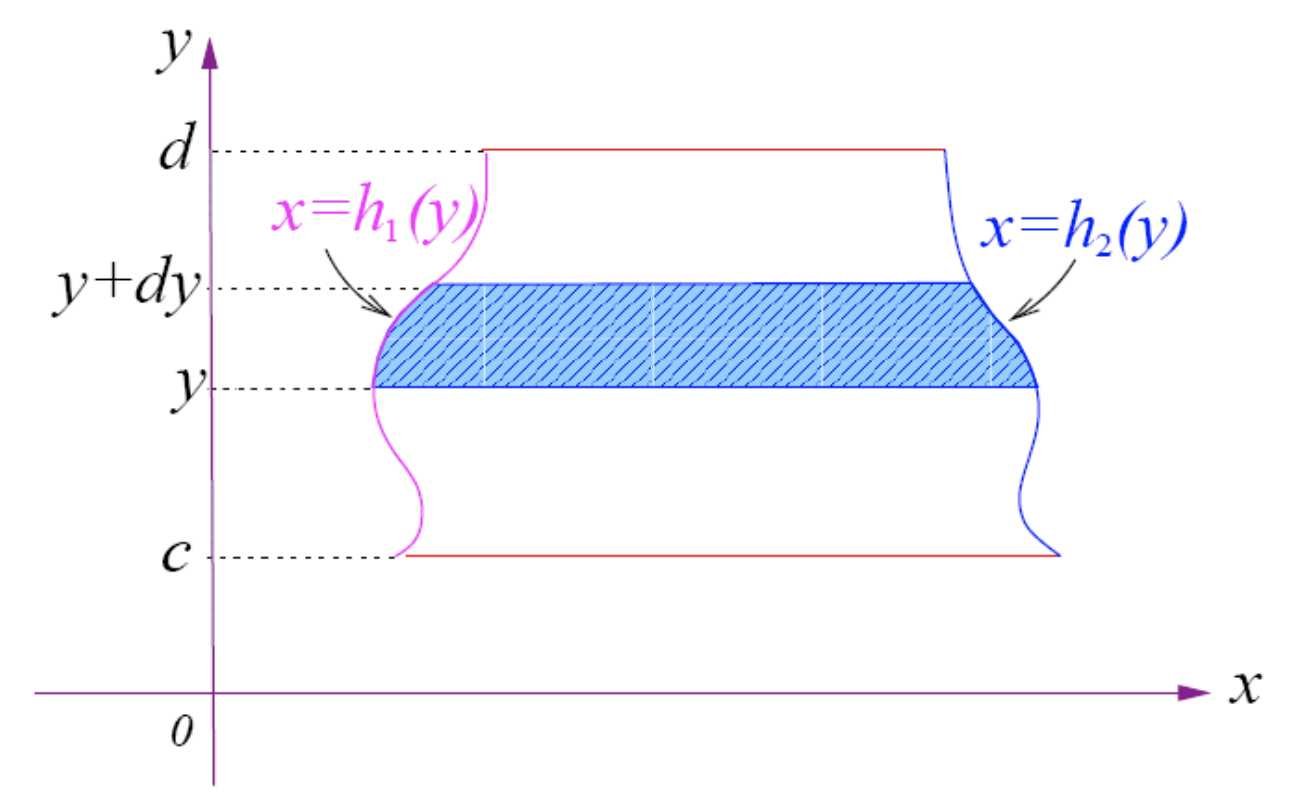
\includegraphics[width=0.9\linewidth]{ma1521-ch7-typeB}
        \\ lower/upper bounds:
        \\* $c \leq y \leq d$
        \\ \ 
        \\ left/right bounds:
        \\* $h_1(y) \leq x \leq h_2(y)$
    \end{multicols}
    
    The region $R$ is given by
    % \\* $R :c \leq y \leq d, \ h_1(y) \leq x \leq h_2(y)$
    \\* $\displaystyle\iint_R f(x,y) dA = \int^d_c\Big [ \int^{h_2(y)}_{h_1(y)}f(x,y)dx \Big ]dy$
\end{center}

\subsection{Polar Coordinates}
\begin{center}
    \begin{multicols}{2}
        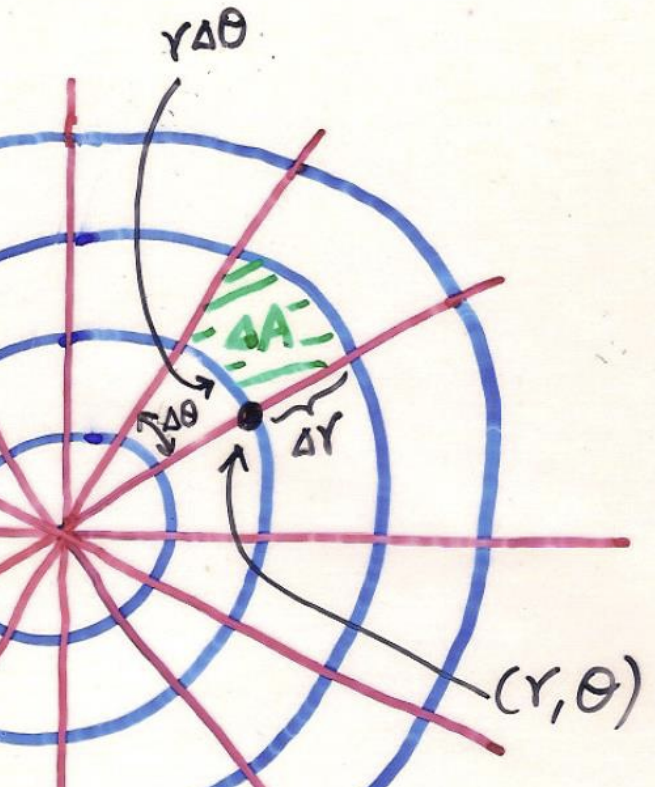
\includegraphics[width=0.85\linewidth]{ma1521-ch7-polar}
        \\ $x = r\cos\theta$
        \\* $y = r\sin\theta$
        \\* $dxdy \Rightarrow rdrd\theta$

        \begin{align*}
            \Delta A &\approx (r \Delta \theta)(\Delta r)
            \\ &= r \Delta r \Delta \theta
        \end{align*}
        % $dA = rdrd\theta$
        \fbox{$dA = rdrd\theta$}
    \end{multicols}
    The region $R$ is given by
    \\* $R: a \leq r \leq b, \ \alpha \leq \theta \leq \beta$
    $\displaystyle\iint_Rf(x, y) dA = \int^\beta_\alpha \int^b_a f(r \cos \theta, r \sin \theta)r\ drd\theta$
\end{center}

\subsection{Applications}
\subsubsection{Volume}
\begin{center}
    Suppose $D$ is a solid under the surface of $z = f(x, y)$ 
    \\* over a plane region $R$
    \\* Volume of $\displaystyle D = \iint_R f(x, y)dA$
\end{center}

\subsubsection{Surface Area}
\begin{center}
    % If $f$ has continuous first partial derivatives on a closed region $R$ of the $xy$-plane, 
    For area $S$ of that portion of the surface $z = f(x, y)$ 
    \\* that projects onto $R$,
    \\* $\displaystyle S = \iint_R \sqrt{(\frac{\partial z}{\partial x})^2 + (\frac{\partial z}{\partial y})^2 + 1} dA$
\end{center}

\section{08. ORDINARY DIFFERENTIAL EQUATIONS}
\begin{itemize}
    \item \textbf{general solution}: solution containing arbitrary constants
    \item \textbf{particular solution}: gives specific values to arbitrary constants
    \item the general solution of the $n$-th order DE will have $n$ arbitrary constants
\end{itemize}

\subsection{Separable Equations}
\begin{center}
    A first-order DE is \textbf{separable} if it can be written in the form 
    \\* $M(x) - N(y)y' = 0$ \quad or \quad $M(x)dx = N(y)dy$
\end{center}

\subsection{Reductions to Separable Form}

\begin{center}
    \def\arraystretch{1.5}
    {\setlength{\tabcolsep}{1em}
    \begin{tabular}{|>{\color{black}}c | >{\color{black}}c|}
        \hline
        form & change of variable
        \\ \hline
        \rule{0pt}{3.5ex}
            $y' = g(\frac{y}{x})$ & \makecell{
                set $v = \frac{y}{x}$ 
                \\ $\Then y' = v + xv'$
            }
        \\ \hline 
        \rule{0pt}{4ex}
            \makecell{
                $y' = f(ax + by + c)$
                \\ $\Then y' = \frac{ax + by + c}{\alpha x + \beta y + \gamma}$
            } & set $v = ax + by$
        \\[2ex] \hline
        \rule{0pt}{3.5ex}
            $y' + P(x)y = Q(x)$ & \makecell{
                $R = e^{\int P dx}$ 
                \\ $\Then y = \frac{1}{R} \int RQdx$ 
                }
        \\[1.5ex] \hline
        \rule{0pt}{6.5ex}
        $y' + P(x)y = Q(x)y^n$ & \makecell{
            set $z = y^{1-n}$
            \\ $\Then y' = \frac{y^n}{1-n} z'$
            \\ $R = e^{\int P dx}$ 
            \\ $\Then y = \frac{1}{R} \int RQdx$ 
        }
        \\[4.5ex] \hline

    \end{tabular}
    }
\end{center}

\subsection{Population Models}
\begin{center}
    $N$ - number; $B$ - birth rate; $t$ - time; $D$ - death rate
    % \\ \      
    \begin{multicols}{2}
        \textbf{Logistic Model}
            $N = \frac{N_{t=\infty}}{1 + (\frac{N_{t=\infty}}{N_{t=0}} - 1)e^{-Bt}}$

        \textbf{Malthus Model}
                $N(t) = N_0e^{kt}$
                \\* where $k = B - D$
    \end{multicols}
\end{center}



\subsection{Common Scenarios}
\textbf{Uranium decays into Thorium}
\begin{tightcenter}
    amount of uranium, 
        \\* $U(t) = U_0e^{-k_Ut}$
        \\* $\frac{dU}{dt} = -k_UU$
    \\* amount of thorium, 
        \\* $T(t) = \frac{k_UU_0}{k_T - k_U}(e^{-k_Ut} - e^{-k_Tt})$
        \\* $\frac{dT}{dt} = k_UU - k_TT$
    \\* decay rate constant, $k = \frac{\ln 2}{t_{1/2}}$
    \\* ratio of thorium to uranium,
        \\* $\frac{T}{U} = \frac{k_U}{k_T - k_U}(1 - e^{-(k_T-k_U)t})$
\end{tightcenter}

\begin{multicols}{2}
    \textbf{Radioactive decay}
    \begin{tightcenter}
        $Q(t) = Q_0e^{-kt}$
        \\* $k = \frac{\ln 2}{t_{1/2}}$
    \end{tightcenter}

    \ \textbf{Cooling/Heating}
    \begin{tightcenter}
        $\frac{dT}{dt} = k(T - T_{env})$
        \\* $\frac{1}{T-T_{env}}dT = kdt$
    \end{tightcenter}
\end{multicols}

\begin{multicols}{2}
    \textbf{Falling objects (N2L)}
    \begin{tightcenter}
        Resistance = $bv^2$
        \\* $m \frac{dv}{dt} = mg - bv^2$
        \\* Let $k = \sqrt{\frac{mg}{b}}$ 
        \\* $\Then \frac{1}{v^2 - k^2} dv = -\frac{b}{m}dt$
    \end{tightcenter}

    \ \textbf{Resistive medium}
    \begin{tightcenter}
        Resistance = $kv$
        \\* $m \frac{dv}{dt} = mg - kv$
        \\* $v' + \frac{k}{m}v = g$ (linear)
        \\ \ 
    \end{tightcenter}
\end{multicols}

\textbf{Concentration of salt in liquid}
\\ Let $R$ = rate of flow (in and out), $Q$ = total amount of salt, 
    \\* $V$ = total volume, $C_{in}$ = concentration of inflow
\begin{tightcenter}
    Rate of flow, $\frac{dQ}{dt} = RC_{in} - \frac{R}{V}Q$
    \\* $\Then Q' + \frac{R}{V}Q = RC_{in}$
\end{tightcenter}

\end{multicols*}
\end{document}